\section{Gráficos y análisis}
Para probar la herramienta desarrollada en la primera parte, se analizaron cuatro redes diferentes a partir de las dos fuentes de información, el Modelo Ethernet y el Modelo ARP. 
A continuación se presentan las cuatro LANs analizadas y sus correspondientes resultados. 

\subsection{Digrafos de las redes}

\subsubsection{Red Hogareña}
Como lo indica su nombre, la misma fue tomada en la casa de uno de los integrantes del grupo. Utilizandose la red Wifi se realizaron capturas de los paquetes Ethernet y, además, de los ARP, de acuerdo al modelo correspondiente. La red presentaba pocos dispositivos conectados y enviando y recibiendo información, por lo que permite un mejor análisis del comportamiento de la misma. 

A continuación se presenta un digrafo que muestra el comportamiento de la red para el Modelo ARP. Se presentan en los nodos a los dispositivos con su correspondiente dirección IP y las aristas corresponden a la cantidad de paquetes de tipo Replay o Request que ocurren entre dos host. 


\centerline{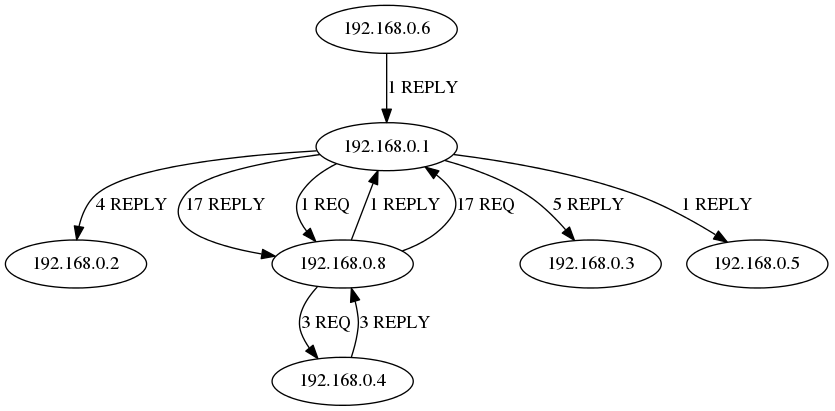
\includegraphics[width=1\textwidth]{./graficos/grafos-arp/grafo_casa_mari.png}}


Como se puede observar, el host con dirección IP 192.168.0.1 se podría comprender que consiste en el router, ya que es el capaz de responder con un mensaje de tipo Replay a todos los mensajes de tipo Request enviados. Luego, en secciones siguientes se podrá distinguir de manera clara cual representaría al nodo distinguido para el evento del Modelo ARP. 

\subsubsection{Red Laboratorio}
En este caso se decidió capturar los paquetes que se encontraban en la red cableada de uno de los laboratorios de la facultad. La cantidad de host que se encuentran interviniendo en la misma es mucho mayor a la de una red hogareña. Se muestra, a continuación, el digrafo generado a partir del evento "una dirección IP participa en el envío de un paquete de tipo Replay o Request a otra dirección IP". 

%Debido al gran número de dispositivos que se involucran en la red, se decidió eliminar aquellos que únicamente participan en el recibimiento o envío de un solo paquete de tipo ARP. Ese filtro se aplica únicamente para la presentación del digrafo del evento "una dirección IP participa en el envío de un paquete de tipo Replay o Request a otra dirección IP".  

\centerline{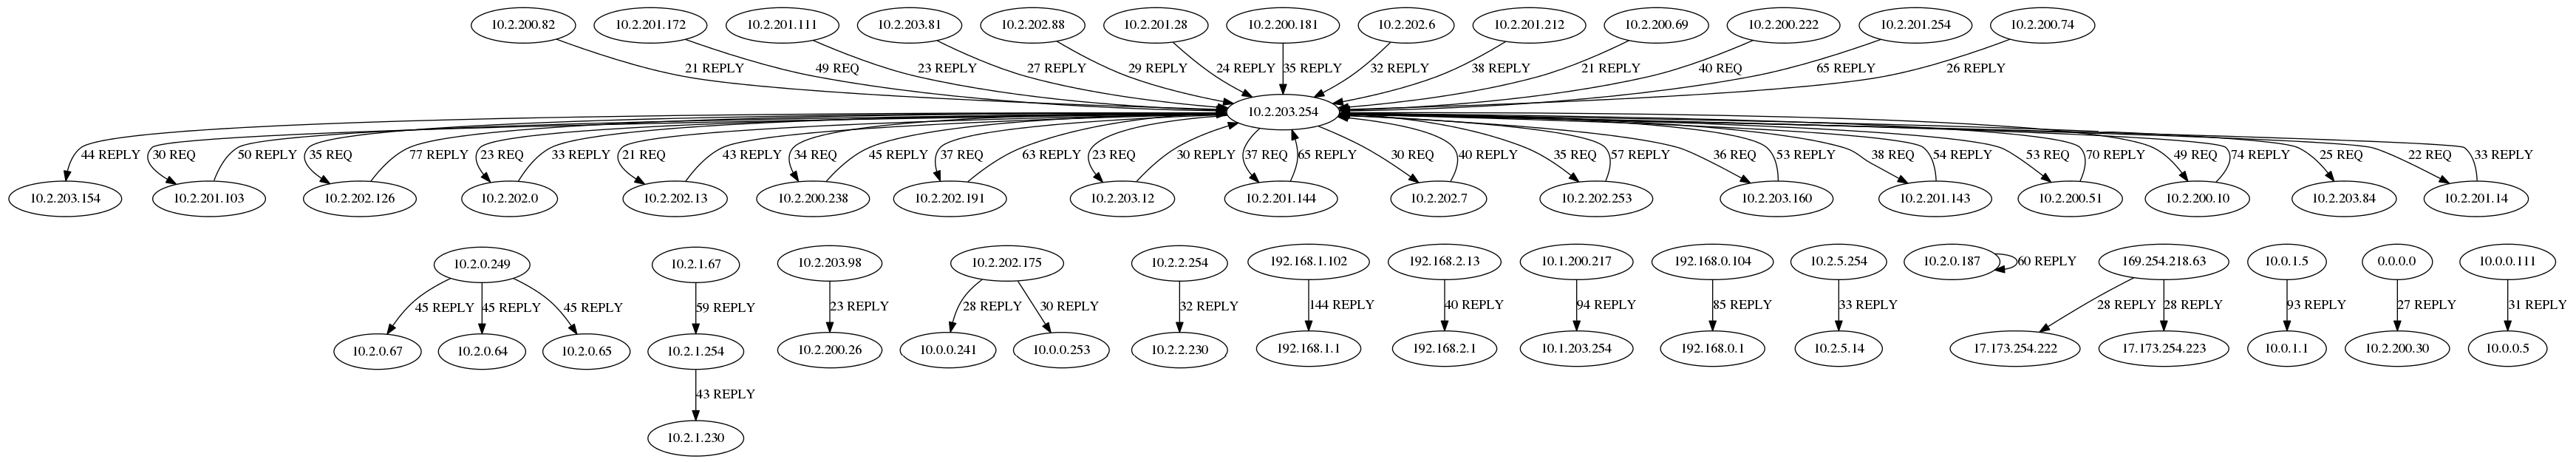
\includegraphics[angle=90, scale=0.3]{./graficos/grafos-arp/grafo_labo5.png}}

A partir del digrafo, se podría concluir que el nodo 10.2.203.254 es un nodo característico debido a la cantidad de información que posee. Luego, mediante otro tipo de análisis, se podrá definir de manera más clara, cual es el nodo característico correspondiente a esa fuente de información para la Red del Laboratorio. 


\subsubsection{Red Devartis}


\subsubsection{Red Mercap}